\chapter{Introduction}\label{chapter:introduction}
Modern computer systems are facing various threats of being attacked. Users are one of the most commonly exploited gateways to computers, especially with social engineering and fishing. Most systems currently rely on a standard combination of username and password. In 2009, Aloul \etal described the most common security concerns with passwords:
``Users tend to use easy-to-guess passwords, use the same password in multiple accounts, write the passwords or store them on their machines, etc. Furthermore, hackers have the option of using many techniques to steal passwords such as shoulder surfing, snooping, sniffing, guessing, etc.'' \cite{aloul2009two} .

Additionally, many users are constantly logged in to services with their mobile devices, despite not having appropriate security measures for their devices. On most Android phones, full disk encryption is not enabled by default \cite{manhattan2015encryption}, which leads to another attack vector for identity theft.

Aloul \etal introduced a system of \glspl{otp} using mobile phones, which significantly improves security by introducing a second factor of authentication. However, for authentication situations on smartphones themselves the \gls{otp} mechanism is rendered pretty much useless, as the second factor is in fact on the same device.

\section{Vision}
The vision of this thesis is to provide a way to easily detect individual users by a short authentication sequence based on acceleration patterns. Even though this does not necessarily qualify as cryptographically secure authentication, behavioural patterns and keystroke recognition can be used as biometric authentication aids. For example, Bhargav-Spantzel \etal \cite{bhargav2006privacy} described a system to extract cryptographic biometric keys from biometric data and showed how this can be combined with additional other proofs of identity to provide strong authentication.

With acceleration pattern recognition, we are able to create an authentication mechanism with zero additional user interaction. This allows higher frequency user re-authentication without disturbing or annoying the user. That means, instead of prompting the user with a login screen every 24 hours, we can measure his or her acceleration patterns every single time sensitive information is accessed. Therefore we can not only provide basic login authentication, but also provide a way for users to stay authenticated for longer sessions or even detect when someone else hijacks a valid session. Since the time between two authentication requests can be arbitrarily small, an attacker who gets control over the current session will be deauthenticated quickly, thus minimizing the potential damage.
\section{Single user licenses}
Another application of this technique is to identify individual users, even when using the same device. This might not only be useful in terms of individualizing the software according to the current user, but also for monitoring software usage.

A common licensing model for software are per-user licenses, \ie $n$ licenses for $n$ users of the software. However, this license model currently can not be enforced since software is installed on a single physical device, which may be shared among users. This led to most software companies licensing their software per-installation instead of per-user.
As of 2016, many users tend to have multiple devices and also want to use their licenses on all of them. This resulted in a trend to bind software licenses to user accounts instead of devices. The trend is also prevailing in modern \gls{saas} models, which do not require installation of the software on end-user devices anymore.
A possible circumvention of these account bound licenses is account sharing. This imposes a real problem, not only for software licensors, but also for other access providers. For example a consumer research from Parks Associates reports, that ``6\% [of video streaming users] are exclusively using shared accounts to access subscription'' \cite{accountsharing}. 

The methods described in this thesis provide a powerful way to detect individual users, sharing physical devices or accounts. Thus with this approach we might reduce copyright infringements that could not be detected beforehand.

\section{Multi-factor authentication}
\gls{mfa} is a technique to enhance security in access control situations. It combines multiple forms of authentication mechanisms, based on conceptually different approaches: Knowledge, \eg passwords or PINs; possessions, \eg keys or bank cards; and biometric characteristics, like fingerprints or behavioural patterns.

A typical authentication attempt with \gls{mfa} is only successful, when all needed factors are present. The most common example for \gls{mfa} is banking, where one individual needs to be in possession of the banking card and also needs to know the card's PIN. However, an attack vector targeting this system is copying the banking card while the attacked person does not notice, that his card is being attacked. This attack vector is also possible with biometric characteristics and even relatively easy, as many biometric traits are publicly visible. Fingerprints have proven to be copyable with low cost \cite{starbug2008bastel} and new high resolution cameras allow to photograph fingerprints and eyes in high enough quality to spoof many scanners \cite{fiebig2014security}. These attacks can be adapted to other authentication systems based on visible biometric traits, such as iris recognition or Android's Face Unlock.

For biometric authentication to be sufficiently secure, the traits need to be intrinsic, \ie not publicly visible and hard to copy. Acceleration based motion detection matches these requirements, as recording of these patterns is only possible with physical access to the authentication device or extremely precise monitoring of all body movement of the user.

\section{Smart mobile devices}
Smart devices are electronic devices, that feature wireless communication, \eg WiFi or Bluetooth. Smart \emph{mobile} devices are smart devices, that are typically worn or kept in close proximity to the user. This usage usually results in small form factors and little weight. These devices are most often commodity devices and used frequently. Therefore, smart mobile devices are ideal to provide authentication, since the authenticating user is accustomed using the device.

\begin{figure}
    \centering
    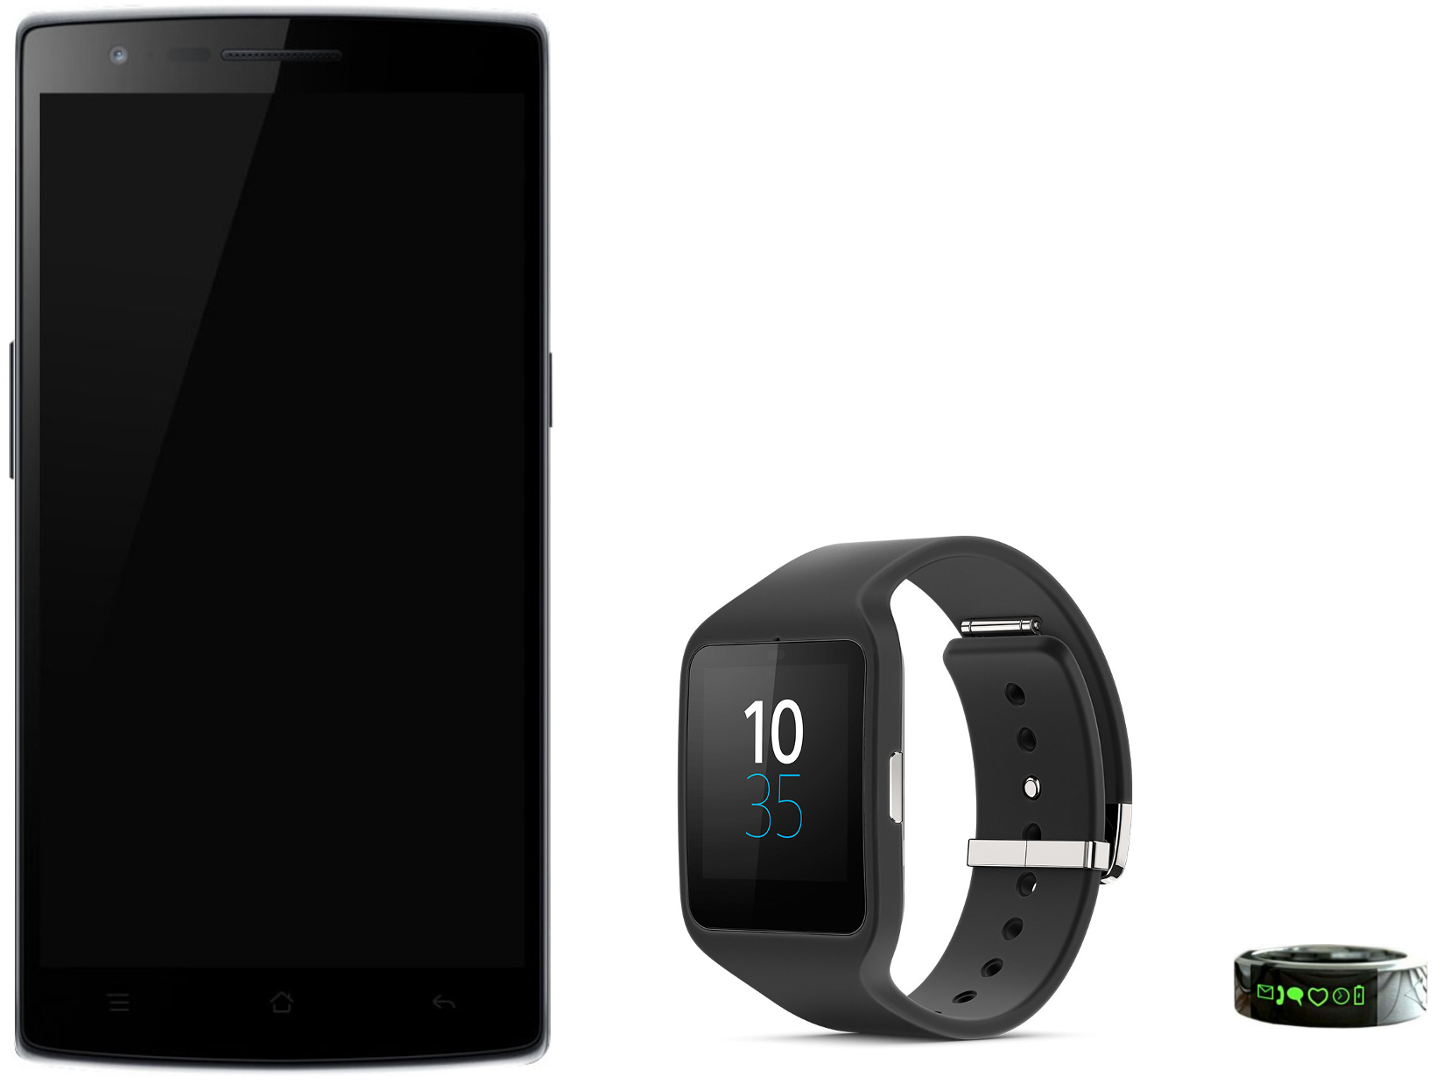
\includegraphics[width=0.7141\textwidth]{figures/SmartDevices.png}
    \caption{Examples for smart mobile devices that are worn in close proximity of the user (from left to right): A OnePlus One smartphone, a Sony SmartWatch 3, Smarty Ring concept design \cite{oneplusone, sonySW3, smartyRing}}
    \label{fig:smartdevices}
\end{figure}
Currently common examples for smart mobile devices are smartphones. With the release of the Apple Watch last year in 2015, smartwatches became increasingly popular. With a rapid miniaturization of smart mobile devices, a consequent next step would be even smaller devices, like smart-rings. In Figure~\ref{fig:smartdevices} a size comparison between the three mentioned categories is shown.

One common trait of almost all smart mobile devices is the presence of acceleration and gyroscope sensors. These sensors are reasonable small and available as integrated circuits to fit in even the smallest devices. For this thesis, we are focusing on acceleration sensors to detect behavioural patterns.

\subsection{Smartphones}
Smartphones are the most capable of the smart mobile devices discussed herein. Smartphones usually have numerous wireless communication possibilities and thus function are a personal data-hub, to which other personal devices connect and communicate over. Typical connections for Smartphones are: Cellular network (\eg \acrshort{gsm}, \acrshort{umts}), WiFi, Bluetooth, Near Field Communication etc. Smartphones are also packed with sensors, which can be utilized in \glspl{app} and typically include acceleration as well as gyroscopic sensors for movement detection.

The three major operating systems of smartphones are Android, iOS and Windows. As shown in Figure~\ref{fig:smartphoneosmarketshare}, Android has the biggest market share of over 80\% and an \gls{app} targeting both Android as well as iOS can reach about 98\% of the smartphone market.

\begin{figure}
    \centering
    \includestandalone[width=0.8\textwidth]{figures/smartphoneosmarketshare}
    \caption{Market share of smartphone operating systems in Q3'15 \cite{gartner2015smartosmarketshare}}
    \label{fig:smartphoneosmarketshare}
\end{figure}

\subsection{Smartwatches}
Smartwatches, as displayed in the middle of Figure~\ref{fig:smartdevices}, are a newer iteration of wearable smart mobile devices. Early designs of smartwatches (essentially calculators) came up in the 1980's and first prototypes were released in the 1990's. However, modern smartwatches feature network connectivity and are usually paired with smartphones via Bluetooth.

\begin{figure}
    \centering
    \includestandalone[width=0.8\textwidth]{figures/wristwearosmarketshare}
    \caption{Market share of wristware operating systems in 2015 \cite{idc2015wristmarketshare}}
    \label{fig:watchmarketshare}
\end{figure}

Currently, the biggest market share, as shown in Figure~\ref{fig:watchmarketshare}, with over 50\% in smartwatches has Apple with the Apple Watch, running watchOS. Android Wear, an adapted version of the Android operating system for smartwatches, has the second highest market share. All in all, the smartwatch market is more diverse than the smartphone market, with several independently developed operating systems like Pebble OS or Samsung's Tizen. Nonetheless, Android Wear has the advantage of having consistent \Glspl{api} with Android. 

With developing \glspl{app} for Android in combination with small adaptions to Android Wear, developers can target a huge percentage of smartphones and also develop smartwatch apps with virtually no overhead.

\subsection{Smart-rings}
Smart-rings are the next step towards even smaller wearables. The concept of these rings is to provide the same basic ``smart'' functionality comparable to a smartwatch, without the need to actually wear a watch. For example displaying notifications or providing authentication for payment processes can also be done solely on a smart ring.

However, there are no commercially available smart-rings yet, but only design concepts and prototypes. Specially developed smart-rings with acceleration sensors should be able to identify users based on their motion patterns. Future work might provide basic functionality on smart-rings, but definitely will need adaption to special purpose operating systems. 

\section{Pattern recognition}
Pattern recognition is a branch of machine learning, that is focused on determining the similarity of datasets. This is usually used to detect predefined patterns, \eg reading numbers or detecting gestures. However, this approach can also be used to generally group similar datasets and classify these without predefined categories. Grouping acceleration patterns is the main goal of this thesis, so pattern recognition algorithms are a main focus.

The pattern recognition concepts and techniques are largely based on Bishop's book ``Pattern Recognition and Machine Learning'' \cite{bishop2006pattern}. We are especially using the concept of a three staged data processing, as shown in Figure~\ref{fig:patternrecognitionsteps}. In this concept, we are first record the raw data, then preprocess it and extract a set of predefined features before using a standard classification algorithm.

\begin{figure}
    \centering
    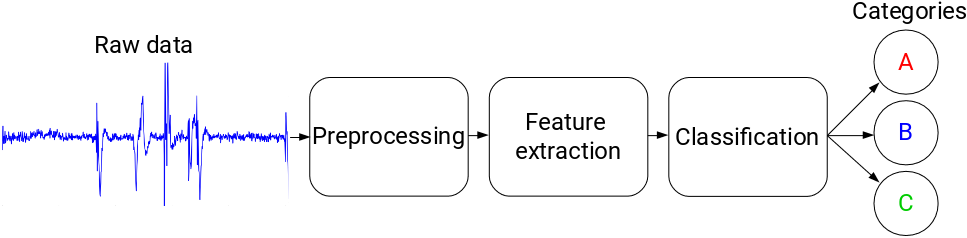
\includegraphics[width=\textwidth]{figures/PatternRecognitionSteps.png}
    \caption{The three staged pattern recognition approach, implemented in this thesis}
    \label{fig:patternrecognitionsteps}
\end{figure}

\subsection{Preprocessing}
In theory, pattern recognition algorithms can work on raw data. However, preprocessing steps can significantly improve the results of these algorithms. In practical applications, preprocessing is used to transform the data, so that the complexity of the problem is reduced. 

A common example using this technique is recognising digits in images. The digit recognition get significantly easier, when the image is cropped to a square around the digit and reduced to a black and white image. Generally speaking, preprocessing steps usually scale the problem to a fixed size and eliminate random noise. As a result, all data is transformed to have similar shape and in general gains predictability.

The preprocessing steps usually operate on the raw input data and do not result in a loss of information.

\subsection{Feature extraction}
The next step, feature extraction, uses more aggressive means to extract the relevant data for our specific use-case. The feature extraction step usually reduces the dataset by several orders of magnitude, which makes subsequent categorization much faster and increases reliability. As a note, we are making a distinction between preprocessing and feature extraction, whereas Bishop \cite{bishop2006pattern} treats them as the same.

Feature extraction is a core component of this thesis, since the performance of the pattern recognition algorithms scales with the amount of data needed to process. The main idea of this step is, that we do not need to compare the whole data from the acceleration sensors, but only ``features'' we identify in the feature extraction step.

However, this feature extraction can also result in information loss. This means, that a precise and accurate feature extraction algorithm is essential. A too broad feature extraction algorithm can result in not recognizing legitimate authentication attempts, while a to narrow algorithm allows attackers to easily bypass this system. Also, for the data to be comparable, all data must undergo the same preprocessing and feature extracting steps. Even slight changes in the algorithms can spoil previous training steps.

\subsection{Classification}
In the end, a pattern recognition algorithm is used to classify the data into various categories. This is usually done by training the algorithm with known categories first. Then, based on this training, the algorithm can decide to which category new data, with a previously unknown category, belongs to. This form of training is called ``supervised'' training.

In general, the training can also be done unsupervised, \ie the initial categories are unknown and the algorithm finds best-fit categories itself. However for this thesis, we implemented a supervised algorithm, which only identifies previously learned users. Automatically recognising new users might be possible as a future enhancement.